\documentclass[11pt]{article}

%\usepackage{sectsty}
\usepackage{siunitx}
\usepackage{tabularx}
\usepackage{float}
\usepackage{graphicx}
\usepackage{mathrsfs}
\usepackage{subcaption}
\usepackage{hyperref}
\usepackage{url}
\usepackage{csquotes}
\usepackage{verbatim}
\usepackage{cite}
\usepackage{stfloats}
\usepackage{textcomp}
\usepackage{algorithm}
\usepackage{algorithmic}
\usepackage{amsmath, amsfonts}
\usepackage{cmsrb}
\usepackage[serbian]{babel}

% Margins
\topmargin=-0.45in
\evensidemargin=0in
\oddsidemargin=0in
\textwidth=6.5in
\textheight=9.0in
\headsep=0.25in

\title{MCP3651 based voltmeter module}

\begin{document}

\maketitle
\pagebreak
\tableofcontents
\pagebreak



\section{Resolution}
MCP3651 ADC has a resolution of 24 bits, however, the 7 ppm max 
INL limits this multimeters count to 146000, just shy of 5.5 digit.

Keeping drift in 1 PPM range, 3 uV drift is acceptable over the 
temperature range.

\subsection{Input current noise limit}
Since for input ranges greater then Vcc the input voltage is feed through
a 10 MOhm divider, input currents noise contribution is:

\section{Input amplifier ideas}

\subsection{NCS21802 only}

\subsubsection{Input current noise at high voltage input}
NCS21802 has 450 \si{\femto \ampere \sqrt{\hertz}}, meaning at input divider
resistance (around 12 kOhm), voltage noise generated is 5.4\si{nV/\sqrt{Hz}}.
At 1 kHz BW, peak to peak noise contribution of input current is 1.02 uVpp.
At 1 Hz, input noise is 32 nVpp.

\subsubsection{Input current noise at low voltage input}

\subsubsection{Input voltage noise}
NCS has 400 nVpp below 10 Hz, while the 1 kHz noise spec of 42 nV/Hz would 
suggest 800 nVpp at that BW. If we use the 1 kHz figure, we can estimate 
1 kHz BW noise is 8 uVpp. At 1 Hz, input voltage noise is 252 nVpp or less.


\subsubsection{Total noise at high voltage input}
Total noise is dominated by voltage noise, which is say 9 uVpp at 1 kHz, 
260 nVpp at 1 Hz. Scaling to input range, 3V signal still has to go into the 
high voltage divider and is reduced to 4.5 mV. 

\subsubsection{IDK}
If we want 500 updates a second, setting the bandwidth to 1000 Hz admits 
1716 nVrms, or 10.3 uVpp of noise.
Reducing the BW to 4 Hz, 0.6 uVpp.

With the proposed 10 Meg, 12.5 k divider, worst case scenario is 3V input voltage,
yealding 3.75 mV across the input divider. In this case, noise reduces the 
voltmeter resolution to 500 counts.


Averaging may improve this noise, but this is garantied to 


\subsection{TL072 and NCS}
TL072 has 80 \si{\femto \ampere \sqrt{\hertz}}, meaning at input divider
resistance (around 100 kOhm), voltage noise generated is \si{8 nV/\sqrt{Hz}}. 
Noise is larger at 0.1 Hz, with peak to peak noise being 300 times larger then
noise density at 1 kHz. Max pp noise is then 2.4 uVpp. 
The input voltage noise pp is 9.2 uVpp.

\begin{equation}
  V_noise = \sqrt{ 9.2^2 + 2.4^2} uVpp = 9.51 uVpp
  \label{eq:NCS218xx input noise}
\end{equation}

In order to retain the 5.5 digit resolution, input range cant go lower than 2V.
At 4.5, input range is 0.2V.

If we want 500 updates a second, setting the bandwidth to 1000 Hz admits 
1716 nVrms, or 10.3 uVpp of noise.
Reducing the BW to 4 Hz, 0.6 uVpp.

With the proposed 10 Meg, 12.5 k divider, worst case scenario is 3V input voltage,
yealding 3.75 mV across the input divider. In this case, noise reduces the 
voltmeter resolution to 500 counts.

\pagebreak

\subsection{Bootstrapped low voltage chopper amplifier input}

\begin{figure}[H]
  \centering 
  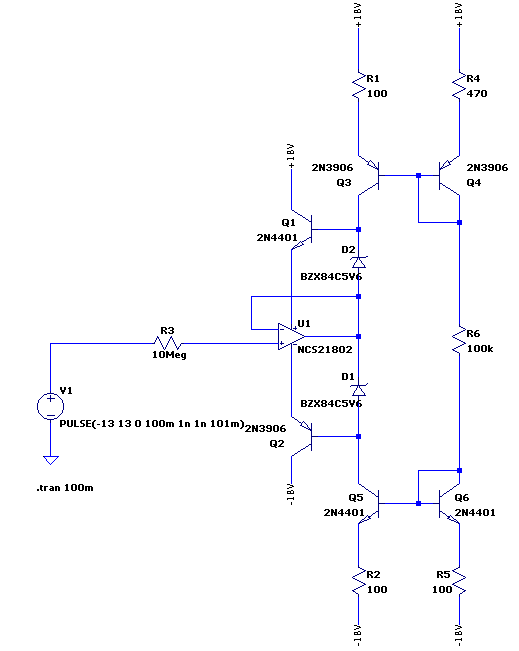
\includegraphics[scale=0.55]{"./figs/bootstrap.png"}
\end{figure}


\section{Calculating errors}

\subsection{Offset drift}

The input stage is TL072 has typical of $\pm 2$ \si{\micro \volt / \celsius} and 
since the input stage features 2, one generating offset, total input 
drift is $\pm 4$ \si{\micro \volt / \celsius}. 

This drift is lowered, as $\pm 10 \si{\volt}$ range gets mapped to 3.3 \si{\volt}
range, meaning the offset drift contribution of TL072 is 
$\pm0.66  \si{\micro \volt / \celsius}$

\begin{figure}[H]
  \centering 
  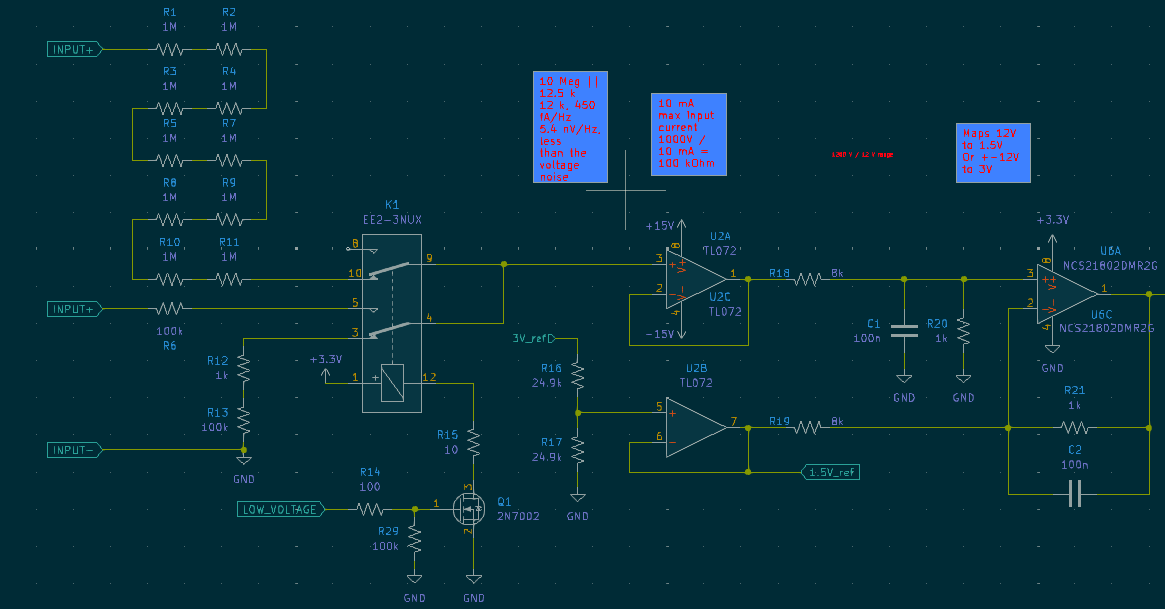
\includegraphics[scale=0.55]{"./figs/Input_amp.png"}
\end{figure}


The second stage consist of two opamps, component NCS21802,
with input offset of $\pm 5$ \si{\nano \volt / \celsius}. First opamp
contributes $\pm 5$ \si{\nano \volt / \celsius}, while second opamps
contribution depends on the selected gain. In the worst case, gain of 
100, the second opamps contribution is $\pm 0.5$ \si{\micro \volt / \celsius}.

The ADC has an input offset drift of $\pm 4$ \si{\nano \volt / \celsius},
meaning the total input offset drift is: 

\begin{equation}
  V_{os} = V_{tl072} + V_{NCS21802} (1 + 100) + V_{ADC}
  \label{eq:offset_1}
\end{equation}

\begin{equation}
  V_{os} = \pm 1.169 \si{\micro \volt / \celsius}
  \label{eq:offset_2}
\end{equation}

Compared to full scale, drift is 0.35 \si{PPM/\celsius},
meaning for a 5.5 digit instrument, the drift is 
les than $\pm1$ LSB for a temperature change of
$\pm 14$ \si{\celsius}.

\subsection{Gain drift}
5.5 digit instruments have 5 PPM resolution.

\pagebreak
\section{Power supply}

\subsection{Mains transformer}
Since leakage is not critical a this stage, +-18V mains transformer should suffice.


\end{document}
